% Fiona Pigott
% March 5 2014

\documentclass[12pt]{article}
\usepackage[margin=1in]{geometry}
\usepackage{amsmath}
\usepackage{amssymb}
\usepackage{graphicx}
\usepackage{float}
\usepackage{multirow}
\usepackage{caption}
\usepackage{subcaption}
\usepackage[T1]{fontenc}
\usepackage{titling}


\setlength{\droptitle}{-3em} 

\title{Adoption Criteria and Network Exposure}
\author{Fiona Pigott}

\begin{document}

%Title
\maketitle

\section*{Goals}
\begin{description}
\item[1:] Discuss different criteria for adopting and maintaining internet use based on adoption data and use case scenarios.
\item[2:] Review network exposure calculations for different formulations and adoption criteria.
\end{description}

\section{Adoption Criteria}

The original data that we have about internet adoption assigns a ``1'' to a node who uses the internet in a given month, and  ``0'' to a user who does not. This results in an unexpectedly high number of \(1 \rightarrow 0\) transitions, which would seem to indicate that it is very common to give up internet service after purchasing it. One possible issue is that until 2003 the only internet service available was dial-up, which charges per minute of internet use. If a node had a dial-up service but did not use it for a month or more at a time, that event would be recorded as a \(1 \rightarrow 0\) transition in the internet adoption data. 

To characterize the recovery behavior that we see here and to see how much these recoveries are affecting the results of the study, we look at the two extreme cases: that all of the \(1 \rightarrow 0\) transitions represent a real recovery and that none of the \(1 \rightarrow 0\) transitions do.
\newpage

\subsection{Original data}
\begin{figure}[h]
    \begin{subfigure}[h]{.55\textwidth}
        \centering
        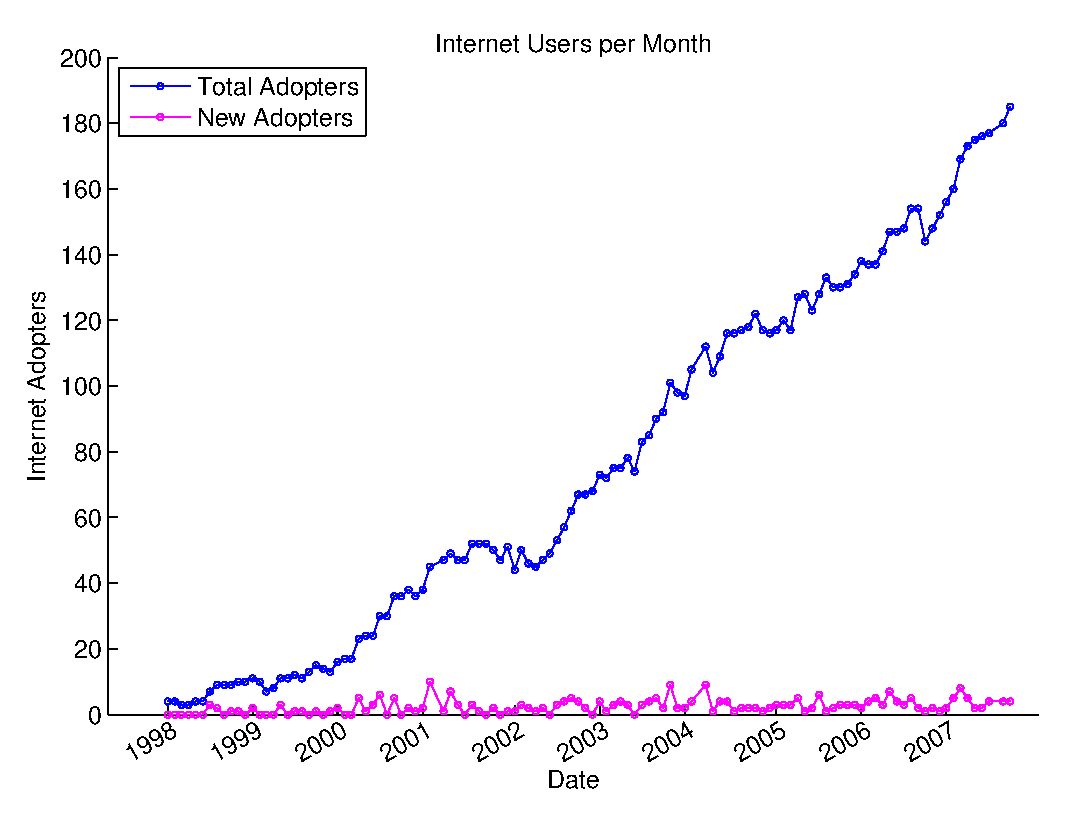
\includegraphics[trim = 2cm 0cm 0cm .5cm, width = .9\textwidth]{Graficos/AdoptersperMonth.eps}
        \caption{Plot showing the number of adopters per month.}% Note that the number of new adopters per month does not change greatly and the number of total adopters grows linearly.}
    \end{subfigure}
    \begin{subfigure}[h]{.55\textwidth}
        \centering
	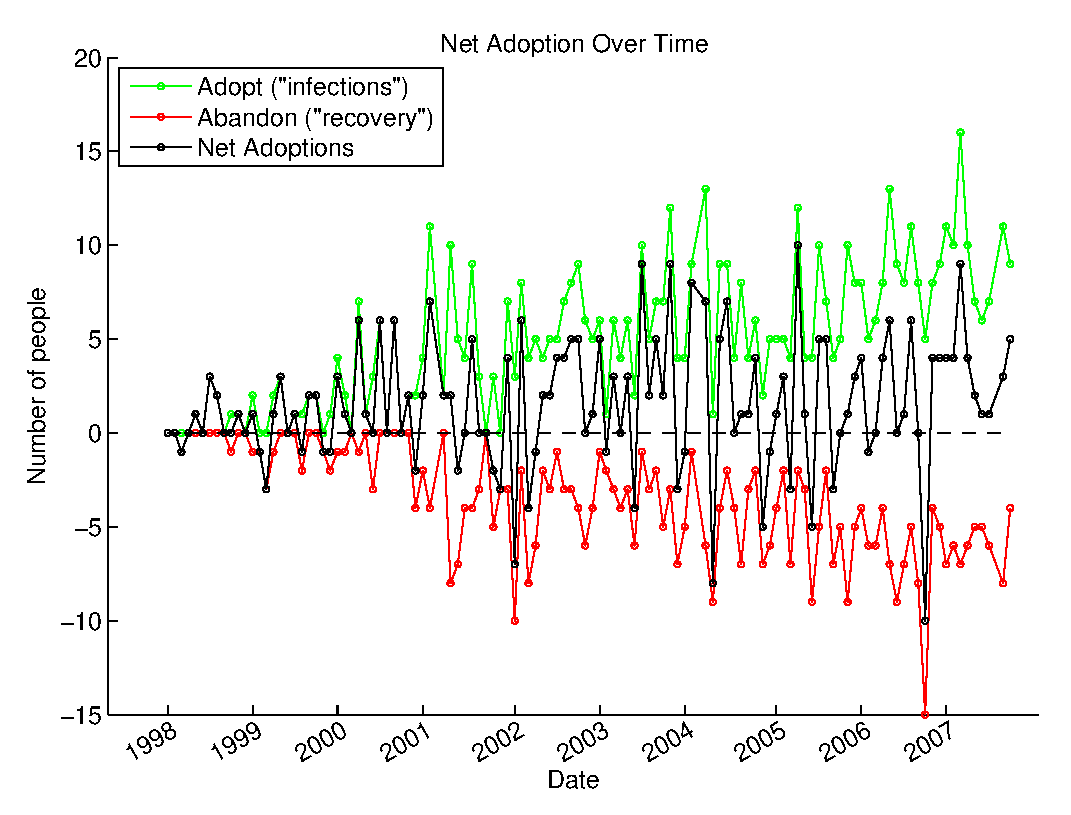
\includegraphics[trim = 2cm 0cm 0cm .5cm, width = .9\textwidth]{Graficos/trans.eps}
        \caption{Fluctuations per month.}% Green shows the number of people who transition from susceptible to infected (S \(\rightarrow\) I), red the number of people who transition from infected to recovered (I \(\rightarrow\) R), and black the net change in the total number of adoptions for the given month.}
    \end{subfigure}
    \caption{Original data showing adoptions over time in the population, where moving from \(0 \rightarrow 1\) is always an adoption (``infection'') and moving from \(1 \rightarrow 0\) is always counted as abandoning internet use (``recovery''), even if the user only abandons internet use for a relatively short period of time.}
\end{figure}

Statistics about the number of transitions that nodes go through:
\begin{table}[H]
\centering
\begin{tabular} {| r  r |}
%\multicolumn{2}{|l|}{\(S \rightarrow I/R\) transitions: } \\ \hline
\hline
Number of nodes who adopt internet at least once: & 286 \\ \hline
Number of nodes who have internet in 12/2007: & 185 \\ \hline
% \% infected nodes who recover at least once: & 63 \% \\ \hline
\% infected nodes who recover for at least: & 1 month: 63 \%\\ 
 & 3 months: 47 \% \\ %\cline{0-1}
 & 6 months: 41 \% \\ %\hline 
 & 12 months: 34 \% \\ %\hline 
\small{(recover for \( >12\) months and not infected by 12/2007)} & permanently: 23 \% \\ \hline 
\end{tabular}
\caption{\(S \rightarrow I/R\) transitions in the network.}
\end{table}

\subsection{Without Recovery}
\begin{figure}[H]
    \begin{subfigure}[t]{.55\textwidth}
       % \centering
        \includegraphics[trim = 2cm 1cm 0cm 1cm, width = \textwidth]{Graficos/AdoptersperMonthP.eps}
        \caption{Plot showing the adopters per month, when \newline adoption is considered a permanent condition. That is, every time a node adopts, that node is considered an adopter permanently.}% Note that the number of new adopters per month does not change greatly and the number of total adopters grows linearly.}
    \end{subfigure}
    ~
    \begin{subfigure}[t]{.55\textwidth}
      %  \centering
	\includegraphics[trim = 2cm 1cm 0.1cm 0cm, width = \textwidth]{Graficos/transP.eps}
        \caption{Fluctuations per month when adoption is permanent. Net adoptions = total adoptions per month, and the number of users abandoning internet use is always zero.}% Green shows the number of people who transition from susceptible to infected (S \(\rightarrow\) I), red the number of people who transition from infected to recovered (I \(\rightarrow\) R), and black the net change in the total number of adoptions for the given month.}
    \end{subfigure}
    \caption{Adoptions over time in the population, where moving from \(0 \rightarrow 1\) is always an adoption (``infection'') but a transition from \(1 \rightarrow 0\) is never counted as abandoning internet use (``recovery'').}
\end{figure}

\section{Network Exposure}

Earlier, we discussed two ways of calculating PNE, or \emph{personal network exposure} for node \(i\) in time step \(m\), a method, definition (\ref{eq:PNE}), which takes into account the network exposure for a node in a given time step \(m\): 

\begin{equation}
{\it PNE}_{{i}} \left( m \right) ={\frac {\sum _{j=1}^{k_{{i}}}
 W_{{i,j}} \left( m \right) Y_{{j}} \left( m-1
 \right) }{\sum _{j=1}^{k_{{i}}}  W_{{i,j}} \left( m
 \right) }}
 \label{eq:PNE}
\end{equation}

or definition (\ref{eq:PNE2}), which takes into account the sum of all network exposure of a node up until a give time step \(m\):

\begin{equation}
{\it PNE}_{{i}} \left( m \right) = {\sum_{n=1}^m \left(  {\frac {\sum _{j=1}^{k_{{i}}}
 W_{{i,j}} \left( n \right) Y_{{j}} \left( n-1
 \right) }{\sum _{j=1}^{k_{{i}}}  W_{{i,j}} \left( n
 \right) } }\right)}
 \label{eq:PNE2}
\end{equation}

It is also possible to calculate PNE using the unweighted (rather than the weighted) graph, in which case definition (\ref{eq:PNE}) becomes:

\begin{equation}
{\it PNE}_{{i}} \left( m \right) ={\frac {\sum _{j=1}^{k_{{i}}}
 A_{{i,j}} \left( m \right) Y_{{j}} \left( m-1
 \right) }{\sum _{j=1}^{k_{{i}}}  A_{{i,j}} \left( m
 \right) }}
 \label{eq:PNEu}
\end{equation}

and definition (\ref{eq:PNE2}) becomes:

\begin{equation}
{\it PNE}_{{i}} \left( m \right) = {\sum_{n=1}^m \left(  {\frac {\sum _{j=1}^{k_{{i}}}
 A_{{i,j}} \left( n \right) Y_{{j}} \left( n-1
 \right) }{\sum _{j=1}^{k_{{i}}}  A_{{i,j}} \left( n
 \right) } }\right)}
 \label{eq:PNE2u}
\end{equation}


for any of the above methods, GNE, or \emph{global network exposure} is simply the sum of the personal network exposure for all nodes for a given month:
 
\begin{equation}
{\it GNE} \left( m \right) =\sum _{i=1}^{N}{\it PNE}_{{i}} \left( m
 \right) 
\end{equation}

Showing a compare/ contrast between the results for each of these methods for both example adoption criteria would be incredibly time consuming, so first, an example for why I chose not to continue working with PNE definitions (\ref{eq:PNEu}) and (\ref{eq:PNE2u}), and instead stick to my original analysis of weighted network exposure calculations.

\begin{figure}[H]
    \begin{subfigure}[h]{.55\textwidth}
        \centering
        \includegraphics[trim = 4cm 1cm 0cm 1cm, height = 7.5cm]{Graficos/GNEperMonthBoth.eps}
        \caption{Comparison of the GNE per month using \newline definition (\ref{eq:PNE}) and definition (\ref{eq:PNE}). The values are \newline practically identical.}

    \end{subfigure}
    \begin{subfigure}[h]{.55\textwidth}
        \centering
	\includegraphics[trim =2cm 1cm 0cm 1cm, height = 7.5cm]{Graficos/GNEvsTotalAdoptersWvsU.eps}
        \caption{Comparison of the graphs of total adopters as a function of GNE using definition (\ref{eq:PNE}) and definition (\ref{eq:PNE}). Once again, this shows very little variation.}
    \end{subfigure}
    \caption{Comparison of weighted network exposure calculations and unweighted network exposure calculations for the original adoption data set and definition (\ref{eq:PNE}) of PNE. Since the strength of a node is linearly related to its degree, on average weight matters very little in these calculations.}
\end{figure}

\newpage

Now, to give an idea about what we are discussing in the next several graphs, these are the two proposed definitions for weighted networks exposure calculations. Both of these are calculated for the original adoption data set only.

\begin{figure}[H]
    \begin{subfigure}[h]{.55\textwidth}
        \centering
        \includegraphics[trim = 4.5cm 0cm 2cm 0cm, height = 7cm]{Graficos/GNEperMonth_def1.eps}
        \caption{Calculating the GNE using definition (\ref{eq:PNE}).}
        \label{fig:GNEdef1}
    \end{subfigure}
    \begin{subfigure}[h]{.55\textwidth}
        \centering
	\includegraphics[trim =2.5cm 1.3cm 2cm 0.5cm, height = 7cm]{Graficos/GNEperMonth_def2.eps}
        \caption{Calculating the GNE using definition (\ref{eq:PNE2})}
                \label{fig:GNEdef2}
    \end{subfigure}
    \caption{Comparison of the calculated network exposure over time using two different definitions for the network exposure on the network. (\ref{fig:GNEdef2}) is simply the integral of (\ref{fig:GNEdef1}), so while the form is different it gives no new information. \newline .}
\end{figure}


\begin{figure}[H]
\includegraphics[trim = 3cm 1.5cm 7cm 2cm, width = .77\textwidth]{Graficos/GNEvsTotalAdopters_GNEdef2.eps}
\caption{Adoption as a function of GNE for definition (\ref{eq:PNE2}) of network exposure, shown for both given criteria for adoption.}
\end{figure}

\newpage

Finally, we can look to see if the network exposure definition substantially changes the relationship between the network exposure of adopters and of non-adopters.

\begin{figure}[H]
    \begin{subfigure}[h]{.55\textwidth}
        \centering
        \includegraphics[trim = 4cm .5cm 0cm 0cm, width = \textwidth]{Graficos/PNEdiffOrig.eps}
        \caption{Network exposure comparison for the original adoption data and definition (\ref{eq:PNE2}) of network exposure. For reference, in 60\% time steps, the PNE of adopters is higher than the PNE of the average population.}
    \end{subfigure}
    \begin{subfigure}[h]{.55\textwidth}
        \centering
	\includegraphics[trim = 2cm .5cm 2cm 0cm, width = \textwidth]{Graficos/PNEdiffP.eps}
        \caption{Network exposure comparison for adoption criteria with no recovery, and definition (\ref{eq:PNE2}) of network exposure. For reference, in 61\% time steps, the PNE of adopters is higher than the PNE of the average population.}
    \end{subfigure}
    \caption{A choice of adoption criteria does not seem to change the overall trend of the network exposure data.}
\end{figure}

The above comparisons motivate the following: that neither the definition of network exposure nor the selection of adoption criteria substantially change conclusions about the network. The graphs below compare adoption as a function of network exposure for both definitions of network exposure and for both adoption criteria choices, and in all cases, the data where node adoption data has been randomly permutated actually shows a higher adoption-to-network exposure slope that the real network and adoption data.



\begin{figure}[H]
\includegraphics[trim = 4cm 1cm 1cm 3cm, width = 1.1\textwidth]{Graficos/GNEvsAdopters_GNEdef1_All.eps}
\caption{Adoption as a function of network exposure for definition (\ref{eq:PNE}) of network exposure.}
\end{figure}

.
\newline .
\newline .

\begin{figure}[H]
\includegraphics[trim = 4cm 1cm 1cm 3cm, width = 1.1\textwidth]{Graficos/GNEvsTotalAdopters_GNEdef2_All.eps}
\caption{Adoption as a function of network exposure for definition (\ref{eq:PNE2}) of network exposure.}
\end{figure}









\end{document}